\documentclass[12pt]{article}

%
%Margin - 1 inch on all sides
%
\usepackage[letterpaper]{geometry}
\usepackage{times}
\geometry{top=1.0in, bottom=1.0in, left=1.0in, right=1.0in}

%
%Doublespacing
%
\usepackage{setspace}
\doublespacing

%
%Rotating tables (e.g. sideways when too long)
%
\usepackage{rotating}


%
%Fancy-header package to modify header/page numbering (insert last name)
%
\usepackage{fancyhdr}
\pagestyle{fancy}
\lhead{} 
\chead{} 
\rhead{Thompson \thepage} 
\lfoot{} 
\cfoot{} 
\rfoot{} 
\renewcommand{\headrulewidth}{0pt} 
\renewcommand{\footrulewidth}{0pt} 
%To make sure we actually have header 0.5in away from top edge
%12pt is one-sixth of an inch. Subtract this from 0.5in to get headsep value
\setlength\headsep{0.333in}

% MLA date format
\usepackage[nodayofweek]{datetime}
\newdateformat{mydate}{\twodigit{\THEDAY}{ }\monthname[\THEMONTH] \THEYEAR}

% include images
\usepackage{graphicx}
\usepackage{float}  % force image placement

% include hyperlinks
\usepackage{hyperref}
\hypersetup{
    colorlinks=true,
    linkcolor=blue,
    filecolor=magenta,
    urlcolor=blue
}
\urlstyle{same}

\begin{document}
\begin{flushleft}

    %%%% First page name, class, etc
    Josie Thompson\\
    Professor Afroditi Psarra\\
    DXARTS 200\\
    \mydate \today\\

\end{flushleft}

\begin{center}
    Hypertext Diagram
\end{center}

The purpose of this art piece is to explore the original meaning of Utopia as it can be interpreted as "good place" or "no place". The piece is what looks like a hyperlink stating "Utopia," but when you click on it, the link literally breaks and the letters fly away from the mouse.\\
The code is written in the lua programming language using \href{https://love2d.org/wiki/Main_Page}{love2d} and can be found here.

\begin{figure}[H]
    \centering
    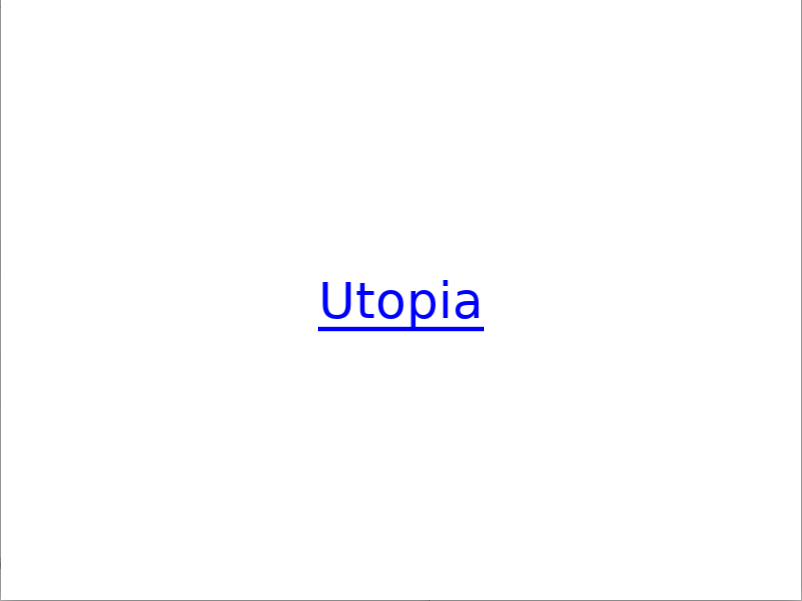
\includegraphics{utopia-2.png}
    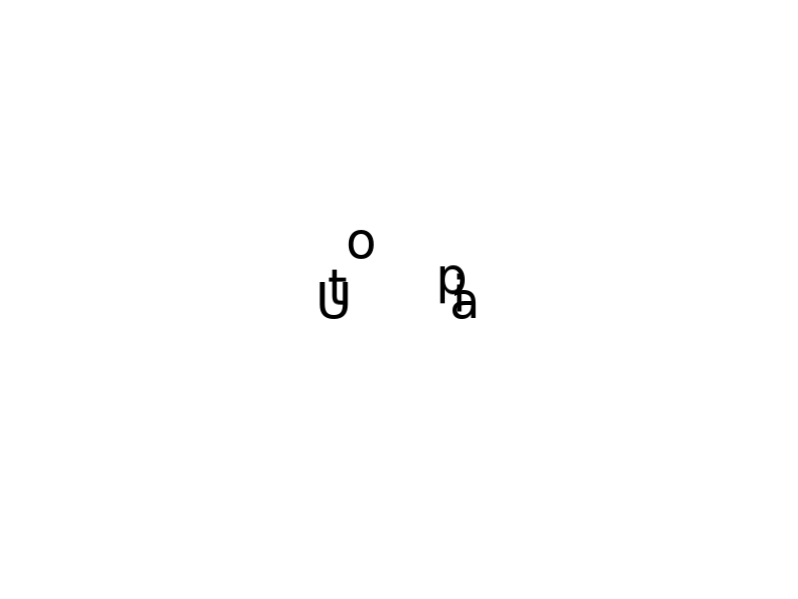
\includegraphics{utopia-3.png}
    \caption{Before and after clicking the link to Utopia}
\end{figure}

\end{document}
